\documentclass[12pt,a4paper]{article}
\renewcommand \baselinestretch{1.5}
\usepackage{booktabs}
\usepackage{textcomp}
\usepackage{amsfonts}
\usepackage{amsmath}
\usepackage{amssymb}
\usepackage{mflogo}
\usepackage[T1]{fontenc}
\usepackage{CJKutf8}
\usepackage[unicode=true,
      CJKbookmarks=false,
      bookmarksnumbered=true,
      bookmarksopen=true,
      bookmarksopenlevel=2,
      breaklinks=true,
      linkcolor=blue,
      plainpages=true,
      pdfpagelabels,
      pdfborder=0 0 0]{hyperref}
%首行缩进
\usepackage{indentfirst}
\usepackage{tabularx}
%图形
\usepackage{graphicx}
\usepackage{subfig}
\usepackage{tikz}
\usetikzlibrary{automata}
\tikzstyle{every state}=[draw=blue!50,very thick,fill=blue!20]
\renewcommand\contentsname{\textbf{目录}}

\author{计研091~黄崇迪~2009210940\\huangcd.thu@gmail.com}
\title{AutomatonConversion项目文档}
\begin{document}
\begin{CJK}{UTF8}{hei}
    \maketitle
\end{CJK}
\begin{CJK}{UTF8}{song}
    \tableofcontents
    \newpage

    \section{项目说明}
    
    \begin{enumerate}
    \item[*] 组号:21(对应GoogleCode中trunk目录下的21Conversion文件夹)
    \item[*] 成员:计研091~黄崇迪~2009210940~hcd05@mails.tsinghua.edu.cn
    \end{enumerate}

    \subsection{项目开发环境}

    \begin{tabular}{r|l}
    \hline
    操作系统 & Windows Vista$^{TM}$ Home Premuim Server Pack 2\\
    CPU & Intel(R) Core(TM)2 Duo CUP P7350 @ 2.00GHz $\times$ 2\\
    内存 & 2.00 GB\\
    JDK版本 & 1.6.0\_13\\
    开发工具 & IntelliJ IDEA 8.1.4\\
    \hline
    \end{tabular}

    \subsection{项目依赖类库}
    项目依赖于JUNG 2.0和Dom4j 1.6两个类库。最多包含下列jar文件:

    dom4j.jar~~collections-generic-4.01.jar~~jung-visualization-2.0.jar

    jung-algorithms-2.0.jar~~jung-graph-impl-2.0.jar~~jung-api-2.0.jar

    concurrent-1.3.4.jar~~stax-api-1.0.1.jar~~colt-1.2.0.jar~~wstx-asl-3.2.6.jar

    \section{程序使用说明(Quick Start)}

    \subsection{基本使用}
    \begin{figure}
    \centering
    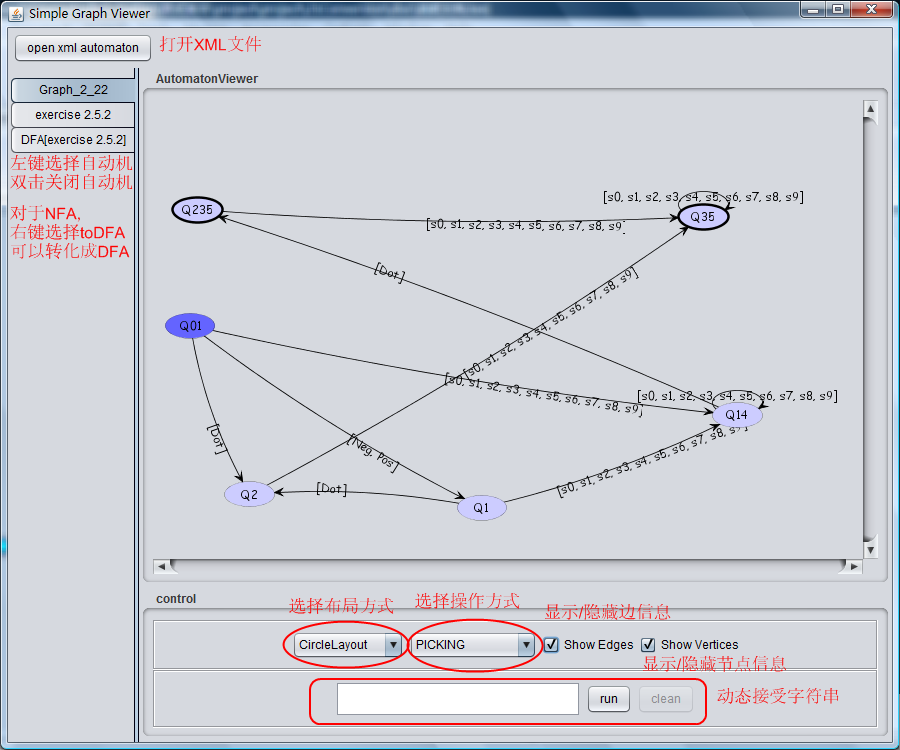
\includegraphics[scale=.4]{full}
    \caption{程序主题界面及简要使用说明}
    \label{fig:full}
    \end{figure}

    通过bin目录下面的run.bat文件或者AutomatonConversion.jar启动程序。
    启动后通过\textbf{open~xml~automaton}按钮打开XML文件。
    图\ref{fig:full}是程序运行某个时刻的截图及各个按钮的简要使用说明。

    AutomatonViewer部分显示自动机,初始状态用深蓝色表示,终止状态用粗框表示,
    其他状态用浅蓝色表示。转换以边的形式表示
    (如果一个状态可以通过多个符号转换成另一个状态,那么图中把多个转移合成为一条边)。

    AutomatonViewer部分支持鼠标中键缩放,图形拖动(TRANSFORMING状态)和节点拖动(PICKING状态)等功能。
    鼠标在节点或者边上悬停出现详细信息。
    也可以选择不同的布局方式(但目前没有效果比较好的布局方式)。

    目前程序的功能主要针对DFA实现。因此对于NFA,动态接受字符串部分不可用,
    但可以通过右键点击标签选择toDFA选项来把NFA转换成DFA。

    \subsection{动态接受字符串}
    目前动态接受字符串只针对DFA实现。使用的方法是在输入框中输入字符串
    (\textcolor{blue}{字符之间需要用“|”分割}),然后点run执行。

    接受过程中,当前状态在AutomatonViewer中显示为黄色,当前符号在输入框中显示为蓝色。
    如果字符串被拒绝,状态和符号都被显示为红色。如果字符串被接受,接受的状态被显示为绿色。

    \section{算法实现及代码介绍}

    \textbf{自动机的表示}

    自动机在程序里面被表示成状态的集合。转移被表示为状态的属性。
        程序里面使用FiniteAutomaton表示抽象的自动机,
        DFA和NFA继承FiniteAutomaton分别表示相应的自动机。
        状态同样对应地有 DFAState和NFAState(实现State接口)。

    \textbf{NFA到DFA的转换}

    根据课本上的算法实现,从初始状态开始根据传递闭包的转移逐步构造整个DFA。
        在NFA.toDFA()函数中实现。

    \textbf{判断自动机是否为空}

    通过广度优先搜索检查从开始状态是否可达终止状态。
        在 DFA.isEmpty() 函数中实现。对于NFA,通过NFA.toDFA().isEmpty()实现。

    \textbf{判断自动机是否为无穷}

    通过深度优先搜索检查从开始状态到终止状态的路径中是否存在环。
        在DFA.isInfinite()函数中实现。对于NFA,通过 NFA.toDFA().isInfinite() 实现。

    \textbf{判断字符串时候被接受}

    根据输入符号遍历状态,字符串结束的时候恰好到达终结状态,
        说明字符串被接受。在DFA.accept()函数中通过调用 DFAState.shift() 实现。
        对于NFA,同样通过 NFA.toDFA().accept() 实现。

    \textbf{XML和自动机的相互转换}

    根据FA.dtd的描述,调用dom4j进行解析或写出。具体实现在
        automaton.io.xml包中的几个类。

    \textbf{显示}

    利用jung实现,具体实现见graph包和ui包。

    \textbf{简单使用例子}

    见sample.Test。
    
    \section{代码量统计(放大查看)}
    \begin{figure}[htbp!]
    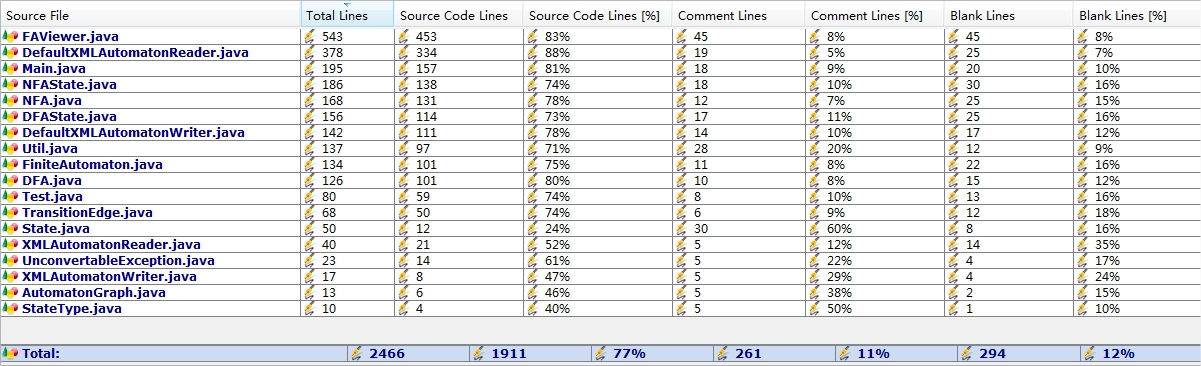
\includegraphics[scale=.32]{Statistic}
    \label{fig:statistic}
    \end{figure}

    \section{项目目标及实现}
    所选项目为\textbf{NFA/DFA的转换工具}。具体要求如下:
    \begin{small}
    \begin{enumerate}
    \item 用Java编写,保证可扩展性。
    \item 检查某个字符串是否被指定的自动机接受。
    \item 判断语言是否为空,是否为无穷。
    \item 实现NFA到DFA的相互转换。
    \end{enumerate}
    \end{small}

    除了实现上述要求内容以外,额外实现了一些功能,具体包括:
    \begin{small}
    \begin{enumerate}
    \item XML到自动机的相互转换
    \item 自动机的可视化及动态接受字符串的过程
    \end{enumerate}
    \end{small}
    
    \section{目前已知的bug}
    当前版本的程序里面,当打开一个NFA,然后右键转换为DFA的时候。
    界面上某个状态可能出现多于1次。初步估计这是Jung库存在的bug(或者是不熟悉Jung的使用导致),
    而与NFA$\rightarrow$DFA转换算法无关。由于这与项目要求没有太多关联,因此这里不做修正,
    而仅仅提供一个折中的方案:每次执行NFA$\rightarrow$DFA的同时,程序将DFA输出到程序所在目录;
    因此可以重新启动一个程序实例打开输出的DFA。
    
    另外,在同一个程序实例里面打开多个自动机实例也可能导致上面问题。
    
    \section{运行结果展示及说明}
    以课本图2.18(xml实例为data目录下的NFA2.xml)为例进行展示:
    
    程序启动以后打开NFA2.xml文件,程序截图如图\ref{fig:NFA},默认的布局方式是CircleLayout,
    相对来说比较清晰。拖动节点(PICKING状态)重新布局得到图\ref{fig:NFA2}。
    \begin{figure}[htbp]
    \centering
    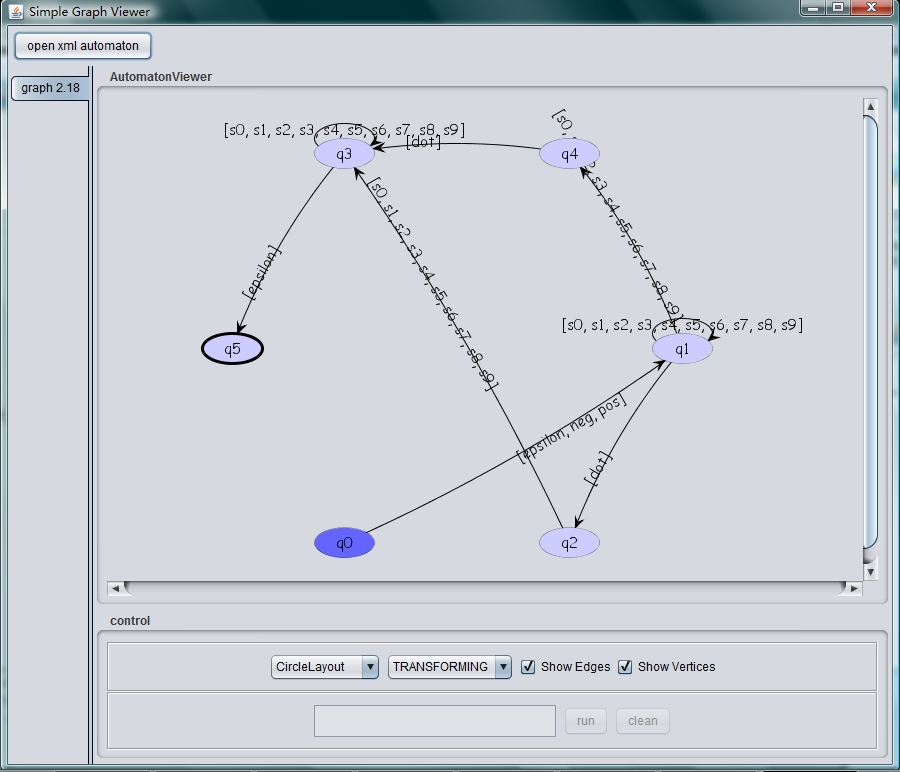
\includegraphics[scale=.3]{NFA}
    \caption{NFA}
    \label{fig:NFA}
    \end{figure}
    \begin{figure}[htbp]
    \centering
    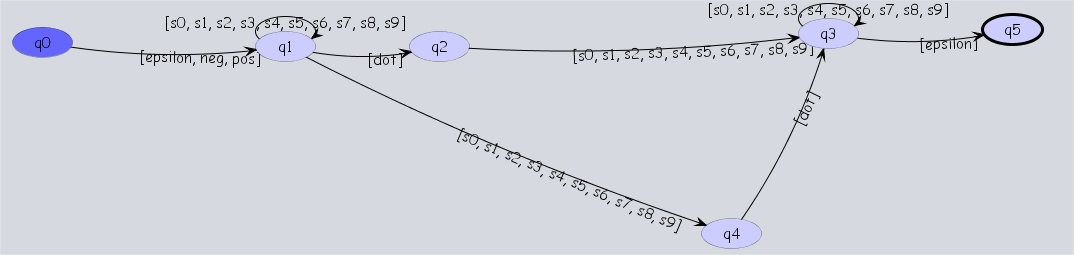
\includegraphics[scale=.35]{NFA2}
    \caption{NFA2}
    \label{fig:NFA2}
    \end{figure}
    
    右键点击标签选择toDFA,然后重新启动程序,打开目录下新生成的DFA[graph 2.18].xml文件,
    拖动节点重新布局得到图\ref{fig:DFA},与课本图2-22比较可以发现,
    图\ref{fig:DFA}仅仅多了一个空状态收集不接受的转移,这说明转移算法是正确的。
    \begin{figure}[htbp]
    \centering
    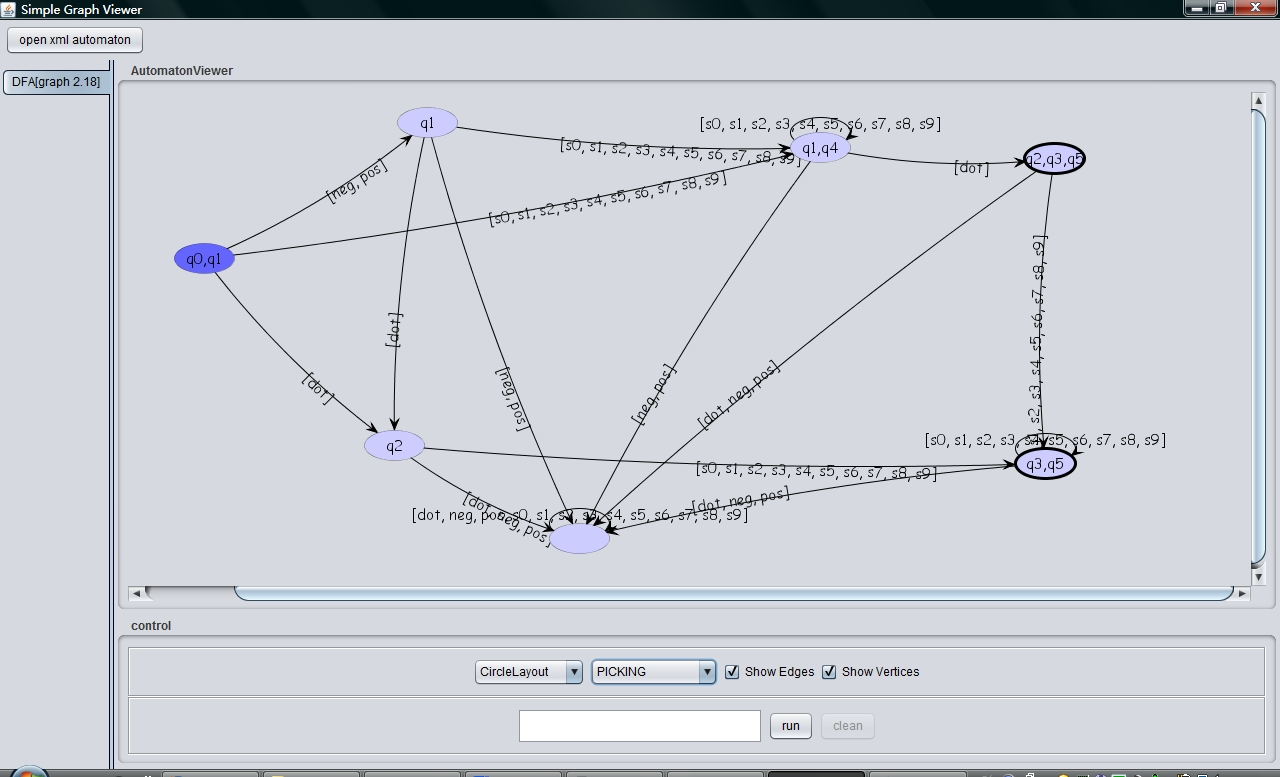
\includegraphics[scale=.3]{DFA}
    \caption{DFA}
    \label{fig:DFA}
    \end{figure}
    
    输入一个正确的例子和错误的例子进行检验:
    \begin{figure}[htbp]
    \centering
    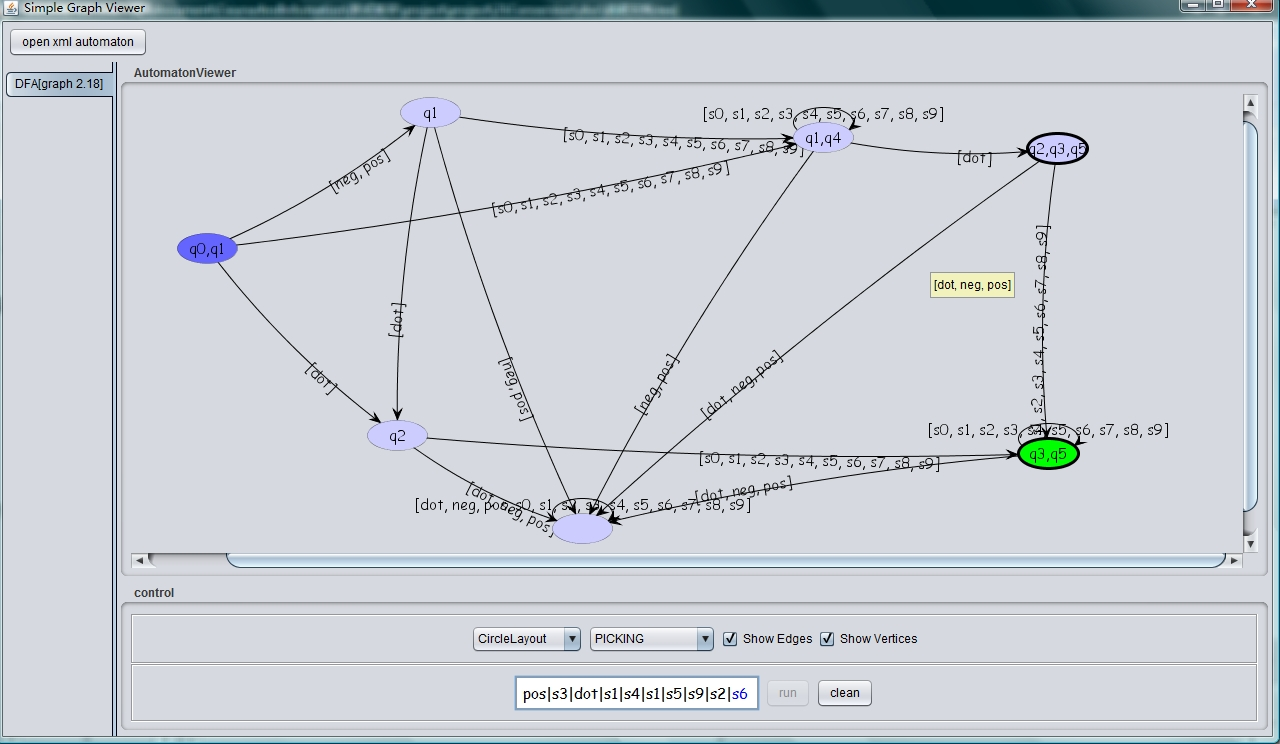
\includegraphics[scale=.3]{correct}
    \caption{正确的例子(+3.1415926)}
    \label{fig:correct}
    \end{figure}
    \begin{figure}[htbp]
    \centering
    
\includegraphics[scale=.3]{error}
    \caption{错误的例子(+-1.231)}
    \label{fig:error}
    \end{figure}
    
    

    \begin{figure}
    \centering
    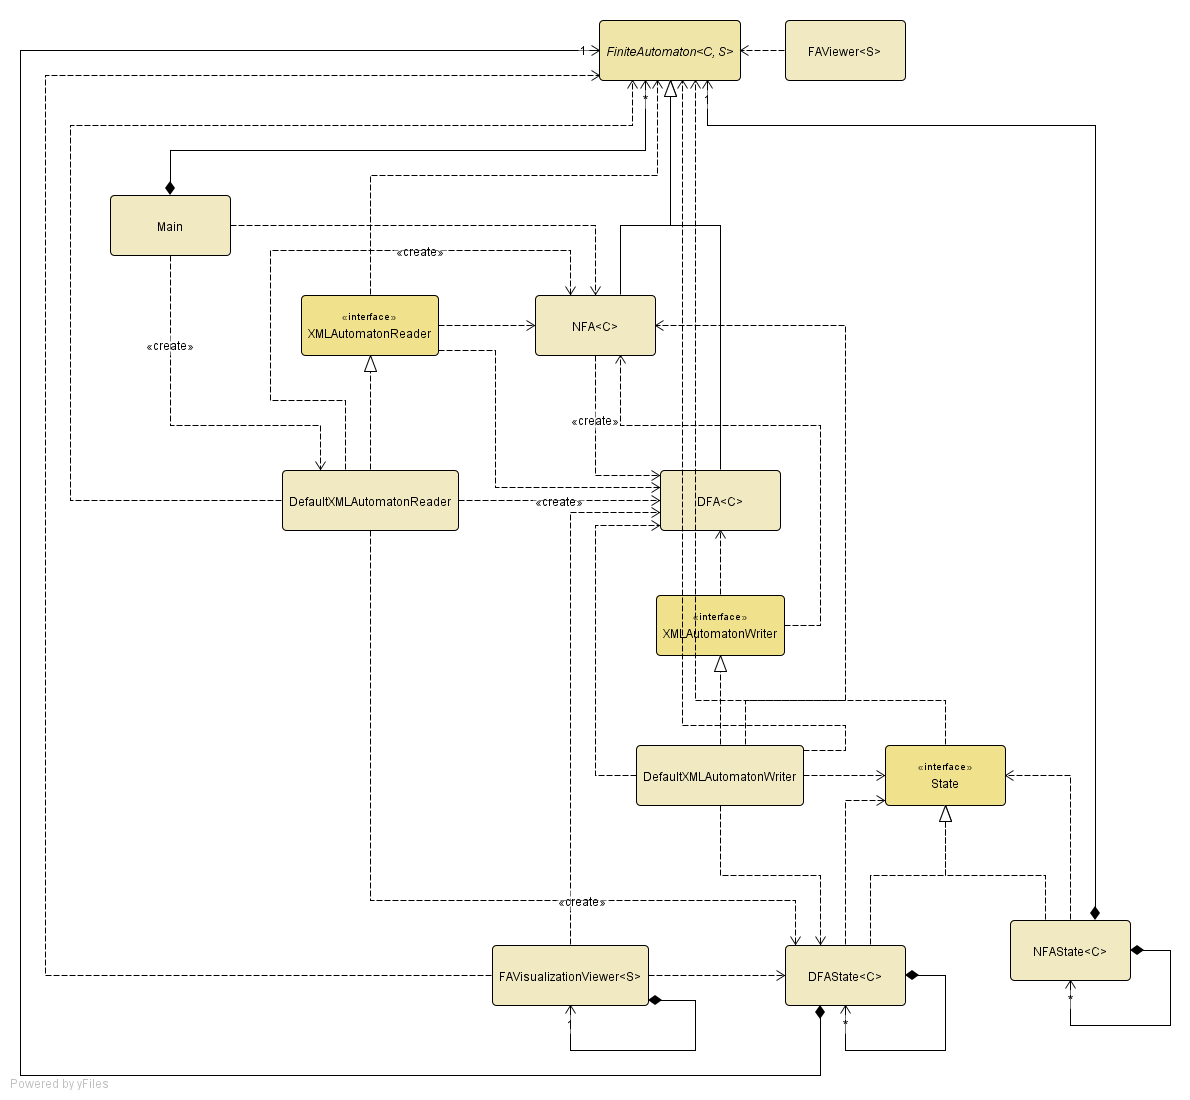
\includegraphics[scale=.3]{UML}
    \caption{各个类之间的关系}
    \label{fig:uml}
    \end{figure}

%这个newpage不能去掉
\newpage
\end{CJK}
\end{document}
